\documentclass[12pt, twoside]{article}
\usepackage[letterpaper, margin=1in, headsep=0.5in]{geometry}
\usepackage[english]{babel}
\usepackage[utf8]{inputenc}
\usepackage{amsmath}
\usepackage{amsfonts}
\usepackage{amssymb}
\usepackage{tikz}
\usetikzlibrary{quotes, angles}
\usepackage{graphicx}
\usepackage{enumitem}
\usepackage{multicol}

\newif\ifmeta
\metatrue %print standards and topics tags

\title{Regents Geometry}
\author{Chris Huson}
\date{September 2020}

\usepackage{fancyhdr}
\pagestyle{fancy}
\fancyhf{}
\renewcommand{\headrulewidth}{0pt} % disable the underline of the header
\raggedbottom


\fancyhead[LE]{\thepage}
\fancyhead[RO]{\thepage \\ Name: \hspace{4cm} \,\\}
\fancyhead[LO]{BECA / Dr. Huson / Geometry 02 Area and volume}

\begin{document}

\subsubsection*{2.6 CW Compound areas, solving for a missing length}
\begin{enumerate}
  \item Find the area $A$ and perimeter $P$ of a square with sides of length 10 centimeters. \vspace{4cm}
    
  \item Find the area $A$ and perimeter $P$ of the shape shown below. The grid is in centimeters.
      \begin{flushleft}
        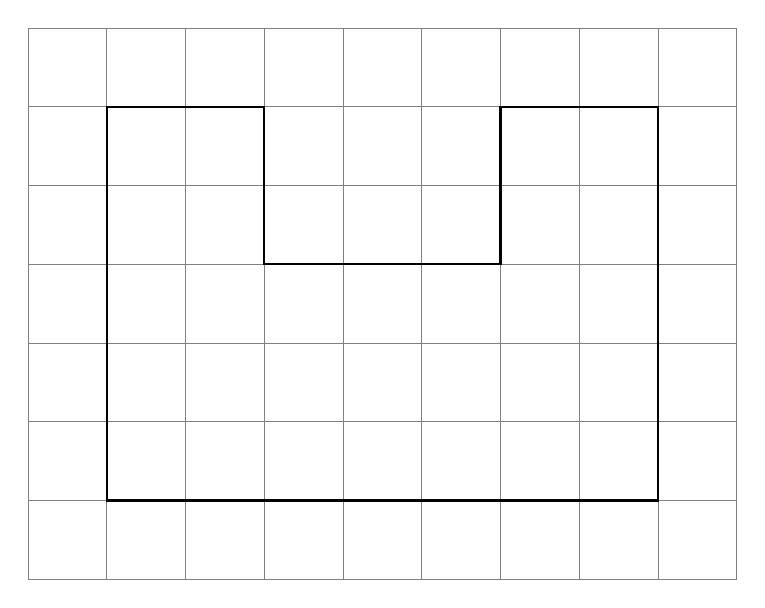
\begin{tikzpicture}[scale=1]
          \draw [help lines] (-4,-4) grid (5,3);
          %\draw [thick, ->] (-2.2,0) -- (10.4,0) node [below right] {$x$};
          %\draw [thick, ->] (0,-2.2)--(0,10.4) node [left] {$y$};
          %\draw (0,0) circle [radius=3] node[below]{$C$};
          %\draw [fill] (0,0) circle [radius=0.05];
          \draw [thick, -] (-3,-3)--(4,-3)--(4,2)--(2,2)--(2,0)--(-1,0)--(-1,2)--(-3,2)--cycle;
        \end{tikzpicture}
      \end{flushleft}
        
  \item The area of a square is 100 square centimeters. Find the length of the side of the square. \vspace{3cm}
      
  \item The perimeter of a square is 100 square centimeters. Find the length of the side of the square.
  
      \newpage
  
  
  \item On the grid below, accurately draw and label two adjacent squares, one with a side length of 4 cm, the other with a side length of 3 cm. The grid is in centimeters.\\*[5pt]
      Find the area $A$ and perimeter $P$ of combined shape.
      \begin{flushleft}
        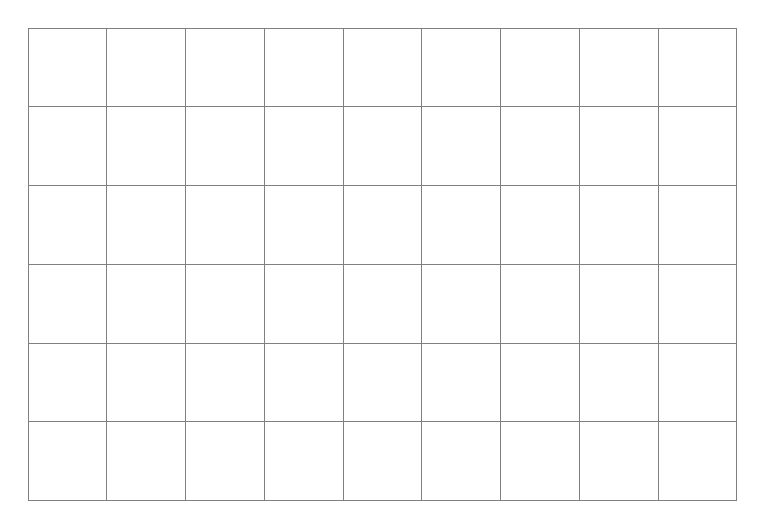
\begin{tikzpicture}[scale=1]
          \draw [help lines] (-4,-3) grid (5,3);
          %\draw [thick, ->] (-2.2,0) -- (10.4,0) node [below right] {$x$};
          %\draw [thick, ->] (0,-2.2)--(0,10.4) node [left] {$y$};
          %\draw (0,0) circle [radius=3] node[below]{$C$};
          %\draw [fill] (0,0) circle [radius=0.05];
          %\draw [thick, -] (-3,-3)--(4,-3);
        \end{tikzpicture}
      \end{flushleft}
  

\item The rectangle $MATH$ has an area of 102, with length $MA=12$. Find the width of the rectangle $AT$.
\begin{flushleft}
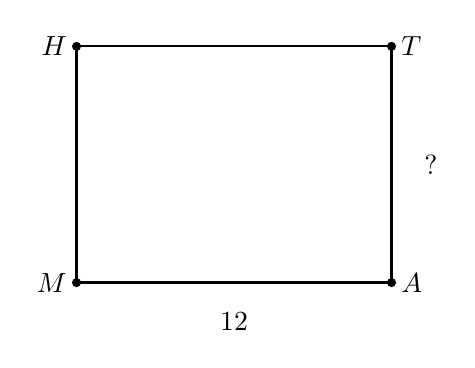
\begin{tikzpicture}
  \draw [-, thick] (0,0)--(4,0)--(4,3)--(0,3)--cycle;
  \draw [fill] (0,0) circle [radius=0.05] node[left]{$M$};
  \draw [fill] (4,0) circle [radius=0.05] node[right]{$A$};
  \draw [fill] (4,3) circle [radius=0.05] node[right]{$T$};
  \draw [fill] (0,3) circle [radius=0.05] node[left]{$H$};
  \node at (4.5, 1.5){?};
  \node at (2, -0.5){12};
\end{tikzpicture}
\end{flushleft} \vspace{1cm} 

  \item One side of the $\triangle ABC$ has a length $AB=8$. The triangle's area is 44. Find the length of the altitude $h$ of the triangle to vertex $C$ and perpendicular to side $\overline{AB}$.\\[0.5cm]
  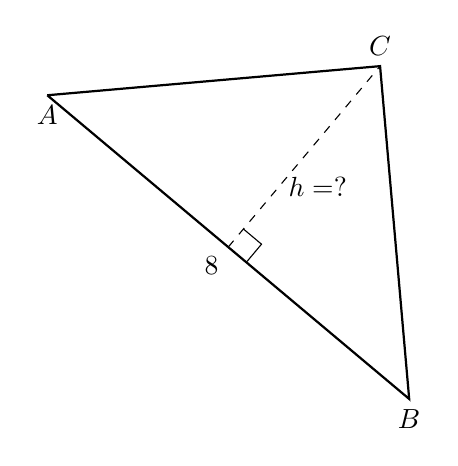
\begin{tikzpicture}[scale=1, rotate=-40]
    \draw [thick]
      (2,0)node[below]{$A$}--
      (8,0)node[below]{$B$}--
      (5,3)node[above]{$C$} --(2,0);
    \draw [dashed] (5,0)--(5,3);
    \draw (5,0)++(0.3,0)--++(0,0.3)--+(-0.3,0);
    \node at (5,1)[right]{$h=?$};
    \node at (5,0)[below left]{$8$};
  \end{tikzpicture}
  
\end{enumerate}
\end{document}